%% =============================================================================
%% SNAPSHOT (read-only archive). Not the live Overleaf source.
%% Recovered from 5090 /home/charlie/project/RecBole/paper_recsys/main_wsdm2027_v3.tex
%% remote mtime: 2026-08-21 18:23 +0800 (yesterday evening).
%% Live files remain: main_wsdm2027_v3.tex and overleaf_deploy/main_wsdm2027_v3.tex
%% (local mtime 2026-08-22 00:19, after the 0821 B1--B10 wording pass).
%% =============================================================================
\documentclass[sigconf,natbib=true,anonymous]{acmart}
%% WSDM 2027 — snapshot 2026-08-21 evening (0821zhidao derisk)
%% Main-table GTS-Last/Random: cutoff-fit, no-cross (Beauty wrap_beauty_*; Toys/Grocery wrap_*).
%% tab:early: matched-protocol Early v2: first 60% train, next 10% valid, next 10% test; last 20% unused.
%% tab:loov: GTS-Last warm, wrap_*_mv, 3-seed mean (2026-08-19).
%% 0820: variants renamed TF / TF+LLM / TF+MV (TF-anchored); tab:shift/tab:bucket =
%%       all-target catalog-level context (not a direct explanation of warm MRR);
%%       hybrid results written in (hybrid_ts_gts_last.csv + random seeds);
%%       cohort counts in 3.1; UniSRec described as adapted backbone; roy2007effective added.
%% 0820: app:intersection = Last/Random on intersecting warm users (gts_intersection_eval.csv,
%%       36 ckpt x 3 sampling seeds); ordering unchanged, so the flip is target selection only.
%% 0821: Early fractions written out (final 20% unused); GTS = interaction cutoff not item-disjoint;
%%       RQ1/RQ2 mechanism sentences demoted to hypothesis; RQ3 redundancy = raw Qwen outputs under
%%       our prompts, not encoder-intrinsic; Fig.1 annotations use ≈ within 1 std.

\settopmatter{printacmref=false}
\renewcommand\footnotetextcopyrightpermission[1]{}
\setcopyright{none}
\acmConference[WSDM'27]{Proceedings of the 20th ACM International Conference on Web Search and Data Mining}{February 15--19, 2027}{Hong Kong}
\acmYear{2027}
\acmDOI{}
\acmISBN{}

\usepackage{booktabs}
\usepackage{multirow}
\usepackage{amsmath}
\let\Bbbk\relax
\usepackage{amssymb}
\usepackage{graphicx}
\usepackage{subcaption}
\usepackage{siunitx}
\usepackage{xspace}
\usepackage{enumitem}
\usepackage{microtype}
\usepackage{balance}
\usepackage{hyperref}
%% Do not hyphenate short function words; prefer geo-metric / sin-gular over geomet-ric / singu-lar.
\hyphenation{under measure geo-metric sin-gular}

\newcommand{\tfidf}{\textsc{TF-IDF}\xspace}
\newcommand{\llm}{\textsc{LLM}\xspace}
\newcommand{\tfllm}{\textsc{TF+LLM}\xspace}
\newcommand{\tfmv}{\textsc{TF+MV}\xspace}
\newcommand{\base}{\textsc{SASRec}\xspace}

\begin{document}

\title{Do More Text Views Help?\\
A Leakage-Aware Evaluation of Text Representations\\
for Sequential Recommendation}

\author{Anonymous Author(s)}
\affiliation{%
  \institution{Anonymous Institution}
  \country{}}
\renewcommand{\shortauthors}{Anonymous}

%==============================================================================
\begin{abstract}
%==============================================================================
%% Abstract claims locked to the submitted text; only variant names unified to TF / TF+LLM / TF+MV.
Text features are widely used to enrich sequential recommenders, but comparisons of lexical \tfidf against TF-anchored LLM augmentations (single-view \tfllm or multi-prompt \tfmv) are often conducted under evaluation protocols that permit temporal overlap.
We conduct a leakage-aware controlled study of ID-only, cutoff-fit \tfidf, \tfllm (a single Qwen2.5-7B view added to the \tfidf base), and \tfmv (four prompt views added to the \tfidf base) under full-ranking global temporal splitting (GTS) on three Amazon datasets, using GTS-Last as the primary protocol, GTS-Random as a robustness check, and clean leave-one-out (LOO) as a contrast.
Three findings emerge.
First, evaluation protocol changes conclusions: across the evaluated settings, text consistently improves over ID-only on warm targets, but the relative ordering of \tfidf, \tfllm, and \tfmv changes across Last, Random, and LOO, even when Last and Random evaluate the same trained checkpoints.
Second, no text representation is robustly dominant across temporal windows; temporal shift reduces absolute performance while preserving near-ties among text variants.
Third, additional prompt views provide limited marginal value because they are highly redundant: inter-view CKA reaches $0.82$--$0.94$, the concatenated representation uses only $53$--$55\%$ of its nominal effective rank, and leave-one-view-out has negligible downstream effect.
In contrast, TF-IDF is geometrically distinct from LLM views (CKA $\approx 0.19$), suggesting a potentially complementary lexical--semantic axis that is not captured by adding more prompt views.
These results suggest that evaluation protocol and representation redundancy should be diagnosed before attributing gains to increasingly complex LLM text pipelines.
\end{abstract}

\begin{CCSXML}
<ccs2012>
 <concept>
  <concept_id>10002951.10003317.10003347.10003350</concept_id>
  <concept_desc>Information systems~Recommender systems</concept_desc>
  <concept_significance>500</concept_significance>
 </concept>
 <concept>
  <concept_id>10002951.10003317.10003318.10003319</concept_id>
  <concept_desc>Information systems~Content ranking</concept_desc>
  <concept_significance>300</concept_significance>
 </concept>
</ccs2012>
\end{CCSXML}
\ccsdesc[500]{Information systems~Recommender systems}
\ccsdesc[300]{Information systems~Content ranking}

\keywords{Sequential Recommendation, Text Features, Temporal Evaluation, Multi-View Redundancy, Leakage-Aware Protocol}

\maketitle

%==============================================================================
\section{Introduction}
\label{sec:intro}
%==============================================================================

Sequential recommendation predicts a user's next item from historical interactions~\cite{kang2018sasrec,sun2019bert4rec,hidasi2016gru4rec}.
Item text---titles, descriptions, and LLM-generated semantics---is a standard way to enrich ID embeddings and enable cross-domain transfer~\cite{hou2022unisrec,bao2023tallrec}.
A natural working hypothesis is that \emph{richer text always helps}: LLM embeddings should beat bag-of-words, and multiple prompt-based views should beat a single view.

This hypothesis is widely held.
Recent work shows that pretrained language representations can improve text-enhanced recommendation and transferability~\cite{hou2022unisrec,li2023recformer,bao2023tallrec}, feature-level attention exploits item attributes and text~\cite{zhang2019fdsa}, and multi-view prompt strategies are increasingly adopted to capture complementary item facets such as function, audience, and style.
Practitioners building production recommenders face a concrete decision: should they invest in LLM inference and multi-prompt pipelines for text features, or does a lightweight bag-of-words baseline suffice?
The answer depends critically on how the comparison is evaluated---a consideration that is seldom examined in text-enhanced recommendation papers.

This hypothesis rests on fragile evaluation foundations.
Most text-enhanced sequential recommenders are validated with leave-one-out (LOO) splits that, as shown by \citet{ji2023evaluation} and \citet{sun2023reevaluation}, allow temporal overlap between training and test, yielding higher absolute metrics and potentially distorting model comparisons.
In a deployment scenario, a recommender must predict items that a user will interact with \emph{in the future}, not reconstruct a randomly held-out historical interaction.
Global temporal split (GTS) better simulates this deployment constraint, but introduces additional design choices: the \emph{target-selection mode} (Last, Random, Successive, or All interactions per user in the test window) itself changes effective task difficulty and can alter model rankings~\cite{gusak2025time}.
Prior work has studied split effects in general~\cite{meng2020temporal,ji2023evaluation}; we show that these effects are \emph{specifically decisive} for the \tfidf vs.\ \tfllm vs.\ \tfmv comparison.

Text features also require preprocessing---vocabulary construction, IDF weighting, SVD projection, and LLM embedding whitening---each of which must respect the temporal boundary.
If these statistics are computed on the full item set (including future items), the resulting features carry information unavailable at training time, introducing a form of leakage orthogonal to the train/test split itself.
We therefore enforce strict \emph{cutoff-fit} controls throughout: all text preprocessing is fit only on items appearing before the training cutoff.

We compare five variants---ID, \tfidf, \tfllm, \tfmv, and an adapted UniSRec baseline~\cite{hou2022unisrec}---on three Amazon datasets under GTS-Last (primary), GTS-Random (robustness check), and clean LOO (contrast), plus an equal-horizon Early temporal window.
We name variants by their full feature composition: the \llm-based variants \emph{augment} the lexical \tfidf base rather than replace it; a base-free LLM-only variant is evaluated separately in Section~\ref{sec:discussion}.
We diagnose multi-view behavior with CKA~\cite{kornblith2019cka}, effective rank~\cite{roy2007effective}, and leave-one-view-out (LOOV).

\smallskip\noindent\textbf{Research questions.}
\begin{enumerate}[leftmargin=*,itemsep=1pt]
\item[\textbf{RQ1}] \emph{Protocol effect.}
Do clean LOO, GTS-Last, and GTS-Random change the absolute gains and relative ranking of \tfidf, \tfllm, and \tfmv?
\item[\textbf{RQ2}] \emph{Temporal robustness.}
Can the conclusions drawn under the Main temporal window ($80\%$ cutoff) survive when the training window shrinks (Early, $60\%$ cutoff)?
\item[\textbf{RQ3}] \emph{Multi-view redundancy.}
Why do four prompt views (\tfmv) not reliably outperform a single view (\tfllm) or even \tfidf alone, and where does potential complementarity lie?
\end{enumerate}

\smallskip\noindent\textbf{Contributions.}
\begin{enumerate}[leftmargin=*,itemsep=1pt]
\item A leakage-aware comparison on three datasets showing that evaluation protocol changes text-representation rankings.  Within GTS, Last vs.\ Random on the same trained checkpoints yields different winners (\textbf{target effect}); switching from GTS to LOO changes both training data and targets (\textbf{split effect}).  Text consistently beats ID, but \emph{which} text is best is protocol-sensitive.
\item Cross-window evidence that no single text variant dominates: under a matched-protocol Early window (first $60\%$ train, next $10\%$ valid, next $10\%$ test; final $20\%$ unused), absolute MRR drops and the Main-window ranking is not preserved, yet text variants remain within 0.001 of each other.
\item A triangulated redundancy analysis (CKA + effective rank + LOOV) spanning raw 3584-d Qwen hidden states through 64-d post-whitening, jointly characterizing limited multi-view gains, while identifying lexical--semantic dissimilarity (TF vs.\ LLM, CKA $0.18$--$0.20$) as a potential complementarity axis.
\end{enumerate}

%==============================================================================
\section{Related Work}
\label{sec:related}
%==============================================================================

\paragraph{Text-enhanced sequential recommendation.}
Early systems fused bag-of-words or review text with collaborative filtering~\cite{wang2015cdl,salton1988termweighting}.
Modern approaches encode titles and descriptions with pretrained language models for cross-domain transfer~\cite{hou2022unisrec,hou2023vqrec,geng2022p5,bao2023tallrec}.
UniSRec learns transferable item representations from text and adapts them via a lightweight MoE~\cite{hou2022unisrec}; VQ-Rec quantizes textual embeddings for transfer~\cite{hou2023vqrec}; P5 casts recommendation as language modeling~\cite{geng2022p5}; TALLRec aligns LLMs to ranking via instruction tuning~\cite{bao2023tallrec}.
These systems typically report LOO or loosely specified temporal protocols.
We do \emph{not} propose a new architecture; we ask whether stronger text encoders and more views remain advantageous once temporal leakage is controlled under a fixed backbone.

\paragraph{LLM-based item representations.}
Beyond architecture papers, a growing practice is to treat LLM embeddings as drop-in item features---either as a single view (title/description) or as multiple prompt-conditioned views that supposedly capture complementary facets (function, audience, style).
This practice is motivated by the intuition that different prompts can elicit diverse semantic aspects of an item (e.g., ``describe the function'' vs.\ ``describe the target audience''), thereby increasing feature coverage.
However, when all views are produced by the \emph{same} pretrained encoder applied to the \emph{same} item text, the diversity of the resulting representations depends on how much the encoder's internal representations actually change in response to different instructions---a question that has received little empirical attention in the recommendation literature.
Our study isolates this representation choice from architectural novelty: the same SASRec backbone and fusion pipeline are held fixed while only the text source changes (\tfidf alone, \tfllm, or \tfmv).

\paragraph{Evaluation protocols and temporal leakage.}
Sampled metrics distort rankings~\cite{krichene2020sampledmetrics}; LOO vs.\ time-based splits change absolute scores and can alter model selection~\cite{ji2023evaluation,sun2023reevaluation,meng2020temporal}.
\citet{hidasi2018recurrent} showed that seemingly minor protocol choices can cause large shifts in relative rankings of sequential models.
Within GTS, target-selection mode matters: \citet{gusak2025time} show that Successive best approximates online next-item prediction but is expensive; Last is a deterministic low-cost proxy; Random has the highest rank-correlation with Successive (we average three sampling seeds because Random is non-deterministic); and All packs multiple items into one ground-truth set, introducing task mismatch and the weakest correlation with Successive.
Beyond sequential recommendation, the impact of temporal protocols has also been documented in session-based~\cite{hidasi2018recurrent} and general collaborative filtering settings~\cite{meng2020temporal}, confirming that protocol sensitivity is not a niche issue but a systemic concern across recommendation paradigms.
We specialize this finding to text representations: protocol changes conclusions \emph{precisely because} \tfidf, \tfllm, and \tfmv respond differently to distribution shift.
Matching validation and test target modes (both Last, or both Random) is also recommended for reliable model selection~\cite{gusak2025time}; our Early-window experiments keep this alignment.

\paragraph{Multi-view learning and representation redundancy.}
Multi-view theory holds that views must be \emph{useful and complementary}; more views do not guarantee benefit~\cite{xu2013multiview}.
In computer vision, \citet{kornblith2019cka} introduced CKA (Centered Kernel Alignment) to measure representational similarity of Gram structures across network layers and architectures; it can detect structural redundancy even when instance-level pairwise cosine is moderate or near zero.
In NLP, \citet{ethayarajh2019contextual} revealed that contextual word embeddings from different layers of the same pretrained model are highly anisotropic and occupy a narrow cone in embedding space, a form of geometric redundancy.
Effective rank (the entropy of normalized singular values)~\cite{roy2007effective} provides a complementary diagnostic, quantifying how much of a representation's nominal dimensionality is actually used.
These tools have been applied to analyze network depth~\cite{kornblith2019cka} and embedding quality~\cite{ethayarajh2019contextual}, but to our knowledge have not been jointly deployed to diagnose \emph{multi-prompt} redundancy in recommendation.
We combine CKA, effective rank, and LOOV---not any single measure alone---to explain limited multi-view gains.

\paragraph{Information geometry of embeddings.}
Singular-value concentration and anisotropy are known failure modes of pretrained text embeddings~\cite{ethayarajh2019contextual}.
When multiple views are generated from the same encoder, these geometric properties propagate: each view inherits similar spectral structure, and concatenation does not proportionally expand the effective subspace.
Our effective-rank analysis connects this literature to sequential recommendation: concatenating four prompt views that share the same encoder yields ER/dim $\approx$0.53, whereas a lexical \tfidf SVD of the same dimension retains ER/dim $\approx$0.98.

%==============================================================================
\section{Controlled Study Setup}
\label{sec:setup}
%==============================================================================

\subsection{Temporal Protocols}
\label{sec:protocol}

\paragraph{GTS-Last (primary).}
Interactions are globally ordered by timestamp.
The \textbf{Main} window uses RecBole's \texttt{TS} split~\cite{zhao2021recbole} $[0.8,0.1,0.1]$: the first $80\%$ of interactions for training, the next $10\%$ for validation, and the last $10\%$ for testing.
After sequential augmentation, each user contributes only their \textbf{chronologically last} test interaction (one target per user)---the deterministic last-item proxy studied by \citet{gusak2025time}.

\paragraph{Early window (RQ2).}
Early uses the first $60\%$ of the globally ordered interactions for training, the next $10\%$ for validation, and the next $10\%$ for testing; the final $20\%$ is unused (RecBole \texttt{TS} $[0.6,0.1,0.1]$; the three fractions are not renormalized to sum to one).
The evaluation window is shifted earlier while validation/test horizon lengths remain fixed at $10\%$ each (equal-horizon with Main).

\paragraph{GTS-Random (robustness check).}
Same checkpoints; each user contributes one \textbf{uniformly random} test interaction.  We average over three target-sampling seeds (42, 123, 456) for stability; cross-seed std per checkpoint is 0.001--0.003.
Random has the highest rank-correlation with Successive~\cite{gusak2025time} and serves as a cross-check.

\paragraph{Clean LOO (contrast).}
Per-user leave-one-out with no global time cutoff: for each user, all but the final two interactions are used for training, the penultimate interaction for validation, and the final interaction for test (RecBole \texttt{LS} split).
Included only to quantify the protocol gap; \emph{not} used for primary conclusions.

\paragraph{GTS-All (appendix).}
All post-cutoff targets per user; relegated to Appendix~\ref{app:gts-all} due to task-mismatch concerns~\cite{gusak2025time}.

\paragraph{Leakage controls.}
\tfidf vocabulary/IDF, SVD projection, and LLM center/whitening are fit only on items appearing before the training cutoff.
Evaluation filters users with $\ge 5$ training interactions.
Main tables report \textbf{warm-target} results: the test target must belong to the training-time item catalog, which is also the candidate set at inference.
Last and Random are evaluated on the \emph{same eligible-user set} per dataset (users passing the min-5 filter with a test-window interaction: Beauty 4{,}520, Toys 4{,}873, Grocery 4{,}152); the two modes differ only in which target interaction is selected.
Because the warm filter applies to the \emph{selected} target, the warm sub-cohort differs slightly between modes (e.g., Beauty: 3{,}137 warm users under Last vs.\ 3{,}054--3{,}083 across Random sampling seeds).
To confirm that this second-order difference does not drive our conclusions, Appendix~\ref{app:intersection} restricts both modes to the intersection of their warm cohorts (users warm under Last \emph{and} under Random): the method ordering is unchanged in every dataset and both modes, so Last-vs.-Random contrasts are target-selection effects on a fixed user population.
All-target and unseen diagnostics appear in Appendix~\ref{app:alltarget}.

\subsection{Text Representations and Models}
\label{sec:models}

All variants share a \base~\cite{kang2018sasrec} backbone ($d{=}256$, 2 layers, 2 attention heads).

\begin{itemize}[leftmargin=*,itemsep=1pt]
\item \textbf{ID}: ID embeddings only.
\item \textbf{TF}: train-cutoff \tfidf $\to$ SVD 256-d $\to$ lightweight projection head + InfoNCE alignment~\cite{oord2018cpc}.
\item \textbf{\tfllm}: the \tfidf base of TF \emph{plus} a single Qwen2.5-7B~\cite{qwen2024qwen25} item embedding (train-cutoff centered and whitened); both sources are fused by the same pipeline.
\item \textbf{\tfmv}: the \tfidf base \emph{plus} four prompt views (Description / Function / Audience / Style) $\to$ per-view 64-d projections $\to$ 256-d concatenation $\to$ shared projection; no cross-attention.
\item \textbf{UniSRec}~\cite{hou2022unisrec}: the original UniSRec architecture (MoE adaptor over item-text embeddings) trained from scratch on each dataset with no cross-domain pretraining; for leakage parity, its item-text inputs are replaced by the same cutoff-fit whitened Qwen2.5-7B embeddings, under the identical evaluation filter.  We therefore treat it as a \emph{UniSRec backbone adapted to our cutoff-fit features}, not as the original pretrained UniSRec.
\end{itemize}

The variant names make the feature composition explicit: the LLM-based variants \emph{augment} the lexical base rather than replace it, so RQ1 compares incremental augmentation of a fixed \tfidf base, not three independent representation families.
A base-free LLM-only variant is evaluated in Section~\ref{sec:discussion}.
All text variants use two-phase training: Phase~A (text-head warmup via InfoNCE), then Phase~B (joint BPR~\cite{rendle2009bpr} + InfoNCE fine-tuning).
Hyperparameters, fusion (no-cross, no boost), and cutoff-fit preprocessing for the Early window are frozen from Main (no re-tuning); the evaluation window is shifted earlier while validation/test horizon lengths remain fixed.

\subsection{Datasets}

Amazon Beauty, Toys \& Games, and Grocery \& Gourmet Food~\cite{mcauley2015amazon,ni2019amazon}:
\begin{itemize}[leftmargin=*,itemsep=1pt]
\item \textbf{Beauty}: 1.21M users, 259K items, 2.02M interactions.
\item \textbf{Toys}: 1.28M users, 336K items, 2.25M interactions.
\item \textbf{Grocery}: 768K users, 172K items, 1.30M interactions (same-platform replication; not claimed as domain diversity).
\end{itemize}

\subsection{Evaluation Details}

Full-ranking Hit@10, NDCG@10, MRR@10~\cite{krichene2020sampledmetrics}.
Main tables: MRR@10, mean$\pm$sample-std over 3 seeds (42, 2024, 2026); NDCG/Hit reported as secondary metrics.
All runs on a single NVIDIA RTX 5090; per-model training: 15--65~min.

%==============================================================================
\section{RQ1: Protocol Changes Rankings}
\label{sec:rq1}
%==============================================================================

\begin{table}[t]
\centering
\caption{%
Protocol contrast --- warm-target MRR@10 (3 training-seed mean$\pm$std, min5 filter; GTS-Random additionally averaged over 3 target-sampling seeds).
\textbf{Bold}: best among the \base-based variants (ID / TF / TF+LLM / TF+MV) per row.
UniSRec is an adapted external baseline and is strongest on Grocery.
Winners change with protocol (point estimates; gaps within one std marked by $\approx$ in Figure~\ref{fig:protocol}): Last favors \tfmv; Random brings TF level with \tfmv; LOO favors \tfllm$\approx$\tfmv$\approx$TF.%
}
\label{tab:protocol}
\small
\setlength{\tabcolsep}{2.2pt}
\begin{tabular}{@{}llccccc@{}}
\toprule
Dataset & Protocol & ID & TF & TF+LLM & TF+MV & UniSRec \\
\midrule
\multirow{3}{*}{Beauty}
 & GTS-Last  & .0032\tiny{$\pm$.0006} & .0053\tiny{$\pm$.0004} & .0060\tiny{$\pm$.0004} & \textbf{.0064}\tiny{$\pm$.0003} & .0052\tiny{$\pm$.0002} \\
 & GTS-Rand  & .0074\tiny{$\pm$.0005} & \textbf{.0124}\tiny{$\pm$.0002} & .0120\tiny{$\pm$.0002} & \textbf{.0124}\tiny{$\pm$.0002} & .0096\tiny{$\pm$.0001} \\
 & LOO       & .0175\tiny{$\pm$.0004} & .0251\tiny{$\pm$.0002} & \textbf{.0254}\tiny{$\pm$.0004} & .0253\tiny{$\pm$.0004} & .0239\tiny{$\pm$.0002} \\
\midrule
\multirow{3}{*}{Toys}
 & GTS-Last  & .0031\tiny{$\pm$.0002} & .0040\tiny{$\pm$.0005} & .0035\tiny{$\pm$.0002} & \textbf{.0042}\tiny{$\pm$.0006} & .0040\tiny{$\pm$.0008} \\
 & GTS-Rand  & .0076\tiny{$\pm$.0002} & \textbf{.0113}\tiny{$\pm$.0004} & .0108\tiny{$\pm$.0007} & .0108\tiny{$\pm$.0009} & .0085\tiny{$\pm$.0003} \\
 & LOO       & .0152\tiny{$\pm$.0005} & .0247\tiny{$\pm$.0006} & .0258\tiny{$\pm$.0012} & \textbf{.0258}\tiny{$\pm$.0028} & .0196\tiny{$\pm$.0010} \\
\midrule
\multirow{2}{*}{Grocery}
 & GTS-Last  & .0030\tiny{$\pm$.0012} & .0046\tiny{$\pm$.0006} & .0047\tiny{$\pm$.0005} & \textbf{.0058}\tiny{$\pm$.0007} & .0107\tiny{$\pm$.0002} \\
 & GTS-Rand  & .0050\tiny{$\pm$.0012} & .0087\tiny{$\pm$.0011} & .0076\tiny{$\pm$.0004} & \textbf{.0089}\tiny{$\pm$.0008} & .0121\tiny{$\pm$.0002} \\
\bottomrule
\end{tabular}
\end{table}

\begin{figure}[t]
\centering
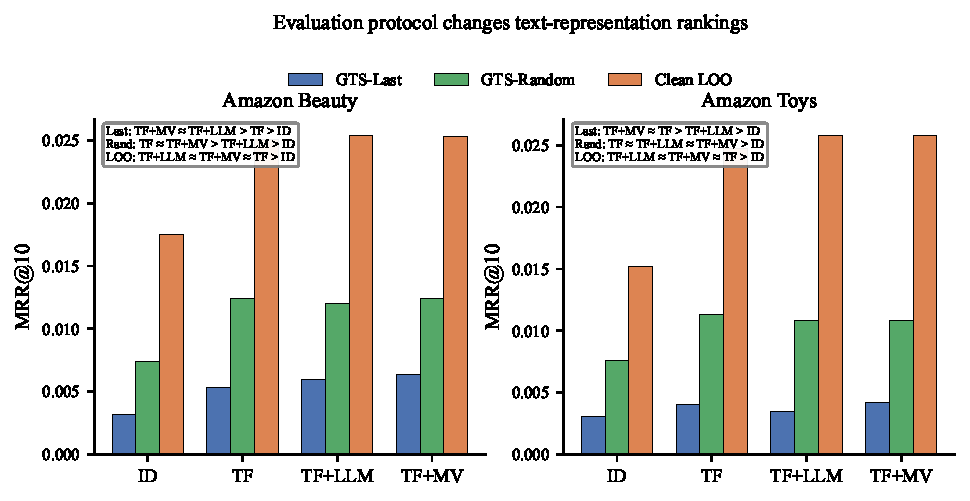
\includegraphics[width=\linewidth]{figures/fig_protocol_contrast.pdf}
\caption{%
Protocol contrast on Beauty and Toys.
Bars are 3-seed \emph{point estimates} (GTS-Last/Random: warm MRR@10; Random further averaged over 3 target-sampling seeds; LOO: clean leave-one-out, contrast only).
In-panel orderings use $\approx$ when the gap is within one seed-level std; they are not a claim of a unique winner.
Last vs.\ Random changes the ordering among the \base-based text variants; LOO raises absolutes and the three text methods are near-ties.%
}
\label{fig:protocol}
\end{figure}

\begin{table}[t]
\centering
\caption{%
GTS-Last warm NDCG@10 and Hit@10 (3-seed mean$\pm$std).
Among the \base-based variants, NDCG agrees with MRR.
UniSRec is strongest on Hit@10 (all three datasets) and on Grocery NDCG.
}
\label{tab:ndcg_hit}
\small
\setlength{\tabcolsep}{2.5pt}
\begin{tabular}{@{}llccccc@{}}
\toprule
Dataset & Metric & ID & TF & TF+LLM & TF+MV & UniSRec \\
\midrule
\multirow{2}{*}{Beauty}
 & NDCG & .0047\tiny{$\pm$.0007} & .0074\tiny{$\pm$.0006} & .0080\tiny{$\pm$.0009} & \textbf{.0087}\tiny{$\pm$.0003} & .0081\tiny{$\pm$.0003} \\
 & Hit  & .0098\tiny{$\pm$.0013} & .0146\tiny{$\pm$.0013} & .0146\tiny{$\pm$.0029} & .0167\tiny{$\pm$.0011} & \textbf{.0180}\tiny{$\pm$.0007} \\
\midrule
\multirow{2}{*}{Toys}
 & NDCG & .0046\tiny{$\pm$.0004} & .0056\tiny{$\pm$.0006} & .0046\tiny{$\pm$.0002} & .0057\tiny{$\pm$.0011} & \textbf{.0066}\tiny{$\pm$.0013} \\
 & Hit  & .0098\tiny{$\pm$.0013} & .0108\tiny{$\pm$.0011} & .0084\tiny{$\pm$.0004} & .0108\tiny{$\pm$.0027} & \textbf{.0154}\tiny{$\pm$.0030} \\
\midrule
\multirow{2}{*}{Grocery}
 & NDCG & .0048\tiny{$\pm$.0019} & .0062\tiny{$\pm$.0004} & .0063\tiny{$\pm$.0005} & .0077\tiny{$\pm$.0007} & \textbf{.0160}\tiny{$\pm$.0003} \\
 & Hit  & .0107\tiny{$\pm$.0041} & .0117\tiny{$\pm$.0009} & .0117\tiny{$\pm$.0007} & .0136\tiny{$\pm$.0007} & \textbf{.0338}\tiny{$\pm$.0007} \\
\bottomrule
\end{tabular}
\end{table}

\begin{table}[t]
\centering
\caption{%
Per-seed GTS-Last warm MRR@10 (seeds 42 / 2024 / 2026).
Variance is visible; \tfmv's lead is small and seed-dependent.%
}
\label{tab:perseed}
\small
\setlength{\tabcolsep}{3pt}
\begin{tabular}{@{}llccccc@{}}
\toprule
Dataset & Seed & ID & TF & TF+LLM & TF+MV & UniSRec \\
\midrule
\multirow{3}{*}{Beauty}
 & 42    & .0038 & .0049 & .0063 & .0063 & .0050 \\
 & 2024  & .0032 & .0052 & .0055 & .0066 & .0054 \\
 & 2026  & .0026 & .0057 & .0063 & .0061 & .0051 \\
\midrule
\multirow{3}{*}{Toys}
 & 42    & .0033 & .0045 & .0037 & .0035 & .0044 \\
 & 2024  & .0030 & .0038 & .0032 & .0042 & .0045 \\
 & 2026  & .0029 & .0036 & .0036 & .0048 & .0031 \\
\bottomrule
\end{tabular}
\end{table}

Table~\ref{tab:protocol} and Figure~\ref{fig:protocol} report the protocol contrast.
No text representation wins everywhere; instead, the relative ordering shifts with the target-selection protocol:

\begin{itemize}[leftmargin=*,itemsep=1pt]
\item \textbf{GTS-Last}: among the controlled \base-based variants, \tfmv is the point-estimate leader on all three datasets (Beauty $.0064$, Toys $.0042$, Grocery $.0058$), but several gaps are within one std (Toys: \tfmv$\approx$TF; Table~\ref{tab:perseed}); the adapted UniSRec baseline is strongest on Grocery ($.0107$).
\item \textbf{GTS-Random} (3 sample-seed avg): TF is the point-estimate leader on Toys ($.0113$ vs.\ \tfmv $.0108$, within one std); Beauty is a tie (TF $.0124$, \tfmv $.0124$); on Grocery \tfmv is ahead by $.0002$ ($.0089$ vs.\ $.0087$), well inside one std.
\item \textbf{LOO}: absolute MRR is 4--7$\times$ higher than GTS-Last; the three text methods are near-ties (\tfllm $\approx$ \tfmv $\approx$ TF).
\end{itemize}
Last vs.\ Random is a \textbf{target-selection} effect on the same trained GTS checkpoints; LOO vs.\ GTS is a \textbf{split/training-protocol} effect (different training data and models).

\paragraph{A plausible account of the LOO gap.}
The 4--7$\times$ higher absolute scores under LOO are not merely an additive shift; they also change the relative ordering among text methods.
LOO permits temporal overlap: a user's training interactions include items from the same time period as the test target, effectively allowing the model to ``memorize'' co-occurrence patterns that would not exist under a strict temporal cutoff.
A plausible explanation is that this overlap disproportionately benefits representations capturing fine-grained semantic similarity (\tfllm and \tfmv), because overlapping items provide richer co-occurrence signal for semantic features than for lexical ones.
Under GTS, where training and evaluation \emph{interactions} are separated by a global temporal cutoff, this advantage is no longer available and the broader lexical coverage of \tfidf becomes competitive.
(Warm evaluation still requires the target item to belong to the train catalog, so the item sets are not temporally disjoint.)

\paragraph{Why do Last and Random disagree?}
Last and Random score the same trained checkpoints on the same eligible users and differ only in which test interaction is selected; the ranking flip survives on intersecting warm users (Appendix~\ref{app:intersection}).
That target-selection effect is the claim~\cite{gusak2025time}.
One plausible hypothesis is that Last and Random draw different mixes of item popularity within the test window, so a representation that ranks higher under one mix need not rank higher under the other.
We do not have a direct statistic showing that Last targets are recently popular, trending, or niche, and we do not claim a lexical-versus-semantic causal mechanism.

\paragraph{Implications.}
The \emph{same checkpoints} (same trained weights), evaluated on the same eligible users, produce different winners when evaluated with Last vs.\ Random target selection---a protocol artifact of target choice.
Claims of text-representation superiority are therefore unreliable without specifying the target mode.
All text methods outperform ID-only under every protocol we evaluate ($+$13--100\% relative under GTS-Last, wider under Random).
Our data thus support a narrow claim (text beats ID) and not a broad one (a single best text representation).

\paragraph{UniSRec as external baseline.}
Under identical GTS-Last + min5 + warm filter, UniSRec scores $0.0052$ (Beauty) and $0.0040$ (Toys), between ID and TF on Beauty and tied with TF on Toys, but it dominates on Grocery ($0.0107$, nearly $2\times$ the next best).
Table~\ref{tab:ndcg_hit} shows that NDCG@10 largely agrees with MRR rankings under GTS-Last, while Hit@10 elevates UniSRec across all three datasets, so metric choice interacts with protocol.
We therefore treat MRR as the primary ranking metric and report NDCG/Hit for completeness.
UniSRec's apparent ranking is protocol-sensitive: dropping the min5 filter inflates GTS-Last MRR into the 0.02 range (Appendix~\ref{app:unisrec}).
The choice of minimum interaction threshold, candidate scope (warm vs.\ full), and target mode can each independently shift where an external baseline appears to rank.

%==============================================================================
\section{RQ2: Temporal Robustness}
\label{sec:rq2}
%==============================================================================

\begin{table}[t]
\centering
\caption{%
Main (first $80\%$ train, next $10\%$ valid, last $10\%$ test) vs.\ Early (first $60\%$ train, next $10\%$ valid, next $10\%$ test; final $20\%$ unused) on Beauty --- GTS-Last warm MRR@10 (3-seed mean$\pm$std).
Fusion and cutoff-fit embeddings matched to Main; hyperparameters frozen.
The Main row matches Table~\ref{tab:protocol}.
Point estimates: \tfmv highest on Main; \tfidf highest on Early (within one std of \tfmv).%
}
\label{tab:early}
\small
\begin{tabular}{@{}lccc@{}}
\toprule
Window & TF & TF+LLM & TF+MV \\
\midrule
Main      & .0053\tiny{$\pm$.0004} & .0060\tiny{$\pm$.0004} & \textbf{.0064}\tiny{$\pm$.0003} \\
Early60-EQ & \textbf{.0042}\tiny{$\pm$.0005} & .0037\tiny{$\pm$.0003} & .0039\tiny{$\pm$.0003} \\
\bottomrule
\end{tabular}
\end{table}

\begin{table}[t]
\centering
\caption{%
All-target catalog-level context (valid$\to$test, Main GTS), \emph{not} a direct explanation of warm-target MRR.
Unseen targets are absent from the train catalog and never enter the warm scores of Tables~\ref{tab:protocol} and~\ref{tab:early}.
Reported as associations with catalog shift, not causal claims.%
}
\label{tab:shift}
\small
\setlength{\tabcolsep}{4pt}
\begin{tabular}{@{}lccc@{}}
\toprule
Dataset & Unseen targets & Pop mean (V$\to$T) & Pop median (V$\to$T) \\
\midrule
Beauty  & 31.9\% & $112.8 \to 101.8$ & $21 \to 15$ \\
Toys    & 40.8\% & $144.7 \to 119.1$ & $18 \to 11$ \\
Grocery & 29.6\% & $87.3 \to 76.9$ & $16 \to 12$ \\
\bottomrule
\end{tabular}
\end{table}

\begin{table}[t]
\centering
\caption{%
All-target popularity-bucket composition (valid$\to$test, Main GTS; head $\ge$10, mid 3--9, low 1--2 train interactions).
Catalog-level context only: unseen items are excluded by the warm filter and do not enter warm MRR.%
}
\label{tab:bucket}
\small
\setlength{\tabcolsep}{3.5pt}
\begin{tabular}{@{}llcccc@{}}
\toprule
Dataset & Split & Head & Mid & Low & Unseen \\
\midrule
\multirow{2}{*}{Beauty}
 & Valid & 63.1\% & 15.9\% & 9.7\% & 11.3\% \\
 & Test  & 56.6\% & 14.9\% & 10.7\% & 17.8\% \\
\midrule
\multirow{2}{*}{Toys}
 & Valid & 60.1\% & 16.3\% & 10.6\% & 13.0\% \\
 & Test  & 52.3\% & 15.5\% & 11.0\% & 21.3\% \\
\bottomrule
\end{tabular}
\end{table}

To isolate the effect of training-window size from test-horizon length, we use an equal-horizon Early split: the first $60\%$ of interactions for training, the next $10\%$ for validation, and the next $10\%$ for testing; the final $20\%$ is unused (RecBole \texttt{TS} $[0.6,0.1,0.1]$).
The evaluation window is shifted earlier while validation/test horizon lengths remain fixed at the same $10\%$ each as Main.

Table~\ref{tab:early} reports GTS-Last warm MRR@10 for both windows under the same no-cross, no-boost, cutoff-fit protocol.
Absolute scores drop from Main to Early for every variant.
The within-window ranking is \emph{not} invariant: the point estimate favors \tfmv on Main and \tfidf on Early ($.0042$ vs.\ \tfmv $.0039$ and \tfllm $.0037$, within one std of \tfmv).
All three remain within $0.001$ of each other.
The Main-window ``\tfmv slightly ahead'' pattern therefore does not survive as a temporal fact.
The Main$\to$Early drop in Table~\ref{tab:early} is measured on warm targets only.
Tables~\ref{tab:shift}--\ref{tab:bucket} provide all-target \emph{catalog-level context} (unseen share, popularity) for the same global cutoffs; they are not a direct explanation of warm-MRR degradation, because unseen items never enter those scores (Appendix~\ref{app:alltarget}).

No single text variant dominates once the temporal window is varied.

\paragraph{Connecting shift to representation type.}
We do not have a per-item statistic that TF-IDF degrades uniformly across items, nor that Last targets are dominated by popular items.
One plausible hypothesis, consistent with Table~\ref{tab:early} where the Main$\to$Early drop is smaller for \tfidf than for \tfllm/\tfmv, is that lexical features and LLM-augmented features respond differently when the evaluation window is shifted earlier.
We emphasize association rather than causation: the catalog-level shift statistics co-occur with the Main$\to$Early drop, but we do not claim that unseen share or popularity shift \emph{causes} the warm ranking pattern.

%==============================================================================
\section{RQ3: Why Limited Multi-View Gain}
\label{sec:rq3}
%==============================================================================

\begin{figure}[t]
\centering
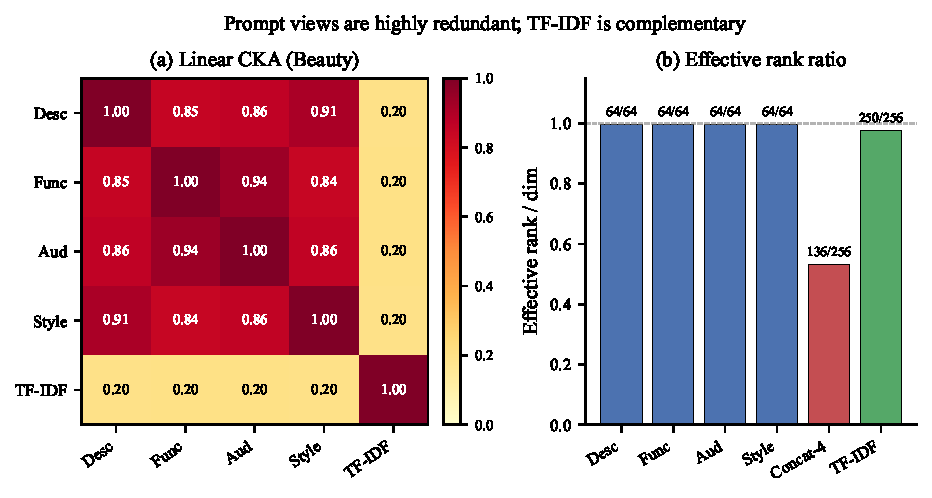
\includegraphics[width=\linewidth]{figures/fig_cka_heatmap.pdf}
\caption{%
Representation analysis on Beauty (3 random item subsamples of 3{,}000 each, mean$\pm$std).
\textbf{(a)}~Pairwise CKA: LLM views show high mutual similarity (0.84--0.94); TF--LLM CKA is low ($\approx$0.20).
\textbf{(b)}~Effective rank: 4-view concat 136/256 (53\%) vs.\ TF-IDF 250/256 (98\%).%
}
\label{fig:cka}
\end{figure}

\begin{table}[t]
\centering
\caption{%
Inter-view CKA (3 subsamples of 3K items, mean$\pm$std).
All LLM view pairs exceed 0.82; TF-IDF vs.\ any LLM view stays within 0.18--0.20.%
}
\label{tab:cka}
\small
\setlength{\tabcolsep}{4pt}
\begin{tabular}{@{}lcc@{}}
\toprule
View Pair & Beauty & Toys \\
\midrule
Description--Function  & $.846 \pm .001$ & $.834 \pm .001$ \\
Description--Audience  & $.860 \pm .001$ & $.856 \pm .002$ \\
Description--Style     & $.914 \pm .000$ & $.904 \pm .001$ \\
Function--Audience     & $.940 \pm .000$ & $.921 \pm .001$ \\
Function--Style        & $.843 \pm .001$ & $.818 \pm .002$ \\
Audience--Style        & $.859 \pm .001$ & $.838 \pm .002$ \\
\midrule
\emph{TF-IDF vs.\ LLM view (range)} & $.196$--$.201$ & $.184$--$.189$ \\
\bottomrule
\end{tabular}
\end{table}

\begin{table}[t]
\centering
\caption{%
Effective rank (Beauty/Toys, 3 subsamples).
4-view concat occupies only 53--55\% of its nominal dimensionality.%
}
\label{tab:effrank}
\small
\begin{tabular}{@{}lccc@{}}
\toprule
Representation & Dim & ER (Beauty) & ER (Toys) \\
\midrule
Single LLM view (avg) & 64 & 63.7 (99.5\%) & 63.6 (99.4\%) \\
4-view concat & 256 & 136.1 (\textbf{53.2\%}) & 141.2 (\textbf{55.2\%}) \\
TF-IDF (SVD) & 256 & 249.9 (97.6\%) & 251.4 (98.2\%) \\
\bottomrule
\end{tabular}
\end{table}

\begin{table}[t]
\centering
\caption{%
Leave-one-view-out (zero-mask, 3-seed mean) under GTS-Last warm, matching Table~\ref{tab:protocol}.
$\Delta$: warm MRR@10 change vs.\ the full 4-view model.
Maximum $|\Delta|$ is 0.00032 (Style on Beauty).%
}
\label{tab:loov}
\small
\setlength{\tabcolsep}{3.5pt}
\begin{tabular}{@{}lccccc@{}}
\toprule
Dataset & Full MRR & $-$Desc & $-$Func & $-$Aud & $-$Style \\
\midrule
Beauty & .00636 & $-$.00021 & $-$.00030 & $-$.00027 & $-$.00032 \\
Toys   & .00417 & $-$.00017 & $+$.00005 & $-$.00007 & $-$.00025 \\
\bottomrule
\end{tabular}
\end{table}

We address RQ3 with three complementary analyses, none of which is sufficient alone: CKA captures structural similarity but cannot by itself prove task-irrelevance~\cite{kornblith2019cka}, effective rank measures dimensionality utilization, and LOOV measures downstream impact.

\paragraph{(1) High inter-view CKA.}
Table~\ref{tab:cka} and Figure~\ref{fig:cka}(a) show that all six LLM view pairs have CKA $\ge 0.82$ (Beauty 0.84--0.94; Toys 0.82--0.92).
The four prompt views, generated from the same encoder applied to the same item text with different instructions, encode highly similar relational structures.
In contrast, TF-IDF vs.\ any LLM view yields CKA 0.196--0.201 (Beauty) and 0.184--0.189 (Toys)---a qualitatively different regime indicating substantial representational dissimilarity.

\paragraph{(2) Pairwise cosine vs.\ CKA.}
Mean pairwise cosine between prompt views is often moderate or near zero (e.g., Description--Function $\approx -0.01$ on Beauty), while Function--Audience reaches $\approx 0.42$.
This does \emph{not} contradict high CKA: cosine measures instance-level alignment of vectors, whereas CKA compares Gram-matrix geometry across the item set~\cite{kornblith2019cka}.
Views can have low average cosine yet still induce nearly isomorphic similarity structures, which is the regime we observe for prompt-based paraphrasing.
We therefore treat CKA as the primary similarity diagnostic and use cosine only as a complementary check, never as standalone proof of redundancy.

\paragraph{(3) Low effective rank of concatenated views.}
Table~\ref{tab:effrank} and Figure~\ref{fig:cka}(b) show that concatenating four 64-d views into 256 dimensions yields effective rank of only 136 (Beauty) and 141 (Toys), occupying 53--55\% of the available capacity.
Nearly half the nominal dimensions carry redundant structure.
TF-IDF at the same 256-d has effective rank $\ge$250 (97--98\%), utilizing almost all capacity.
Concatenating prompt views therefore expands the subspace far less than the dimension count suggests.

\paragraph{(4) Negligible LOOV impact.}
Table~\ref{tab:loov} shows that zeroing any single view has minimal downstream effect under GTS-Last warm: maximum $|\Delta|$ = 0.00032 ($\approx$5\% of the full \tfmv score).
Full MRR matches Table~\ref{tab:protocol}'s \tfmv column.
Per-seed signs can flip, so we do not treat any prompt as uniquely necessary.

\paragraph{Where does redundancy originate?}
To disentangle prompt-induced from preprocessing-induced redundancy, we compare CKA at two stages: \emph{pre-whitening} (SVD-projected + centered, 64-d per view, \textbf{without} ZCA whitening) and \emph{post-whitening} (the final model-input embeddings).
On Beauty, mean pairwise CKA is $0.96\pm0.001$ pre-whitening and $0.88\pm0.001$ post-whitening; on Toys, $0.96\pm0.001$ and $0.87\pm0.001$ respectively.
CKA is \emph{already extremely high before whitening} (Table~\ref{tab:cka-prepost}): whitening \emph{reduces} mean inter-view CKA by 0.08 (Beauty) and 0.10 (Toys), and raises concatenated effective rank from 99/256 (39\%) to 136/256 (53\%) on Beauty and from 104/256 to 140/256 on Toys.

To trace redundancy further upstream, we compute inter-view CKA directly on the raw 3584-d Qwen hidden states \emph{before any SVD projection}.
Mean pairwise CKA at 3584-d is $0.961$ on Beauty and $0.963$ on Toys (3-trial random subsample of 3000 items, $\sigma < 0.002$).
Effective rank of the concatenated 4-view matrix ($4\times 3584 = 14336$-d) is only 1567 (10.9\%) on Beauty and 1622 (11.3\%) on Toys.
Redundancy is therefore already present in the raw Qwen outputs before SVD or whitening \emph{under our prompt design}, rather than an artifact of SVD truncation: the four instruction variants induce near-isomorphic relational structures at 3584-d, and the $\sim$90\% dimensionality collapse is already present at that stage.
This audit cannot separate encoder-intrinsic collapse from using the same item text or from prompts that are insufficiently divergent.
Whitening partially decorrelates the views but cannot remove this structural overlap.
Expanding view dimensionality to $4\times256$ is thus \emph{not} justified---the bottleneck is source redundancy under this prompt design, not projection capacity (Table~\ref{tab:cost}).

\begin{table}[t]
\centering
\caption{%
Pre- vs.\ post-whitening audit (3 item-subsamples, mean).
CKA is already $\ge$0.94 before whitening; whitening lowers CKA and raises concat effective rank, so redundancy is not a whitening artifact.
Subsamples are drawn independently of Table~\ref{tab:effrank}, hence the $\pm 1$ difference in the Toys post-whitening rank.%
}
\label{tab:cka-prepost}
\small
\begin{tabular}{@{}llcc@{}}
\toprule
Dataset & Stage & Pairwise CKA & Concat ER/256 \\
\midrule
\multirow{2}{*}{Beauty}
 & Pre-whiten (SVD+center)  & 0.94--0.99 & 99 (39\%) \\
 & Post-whiten (TS fit)     & 0.84--0.94 & 136 (53\%) \\
\midrule
\multirow{2}{*}{Toys}
 & Pre-whiten (SVD+center)  & 0.94--0.98 & 104 (41\%) \\
 & Post-whiten (TS fit)     & 0.82--0.92 & 140 (55\%) \\
\bottomrule
\end{tabular}
\end{table}

\paragraph{Synthesis.}
The three diagnostics agree: prompt views encode overlapping semantics, which produces dimensionality collapse and negligible per-view contribution.
The observed geometry is consistent with insufficient view complementarity in the sense of multi-view theory~\cite{xu2013multiview} (views derived from a single source via semantic paraphrasing).
The potential complementarity in our system lies between lexical \tfidf and semantic \llm views (CKA $0.18$--$0.20$), suggesting representational dissimilarity that is not harvested by naive multi-prompt stacking: the \tfmv model replicates similar semantic structures four times instead of further exploiting the lexical--semantic axis it already contains.

%==============================================================================
\section{Discussion and Limitations}
\label{sec:discussion}
%==============================================================================

\paragraph{Why does TF-IDF alone match \tfmv?}
Why can a bag-of-words representation match or exceed the four-view variant under GTS-Random?
We see two contributing factors.
First, \tfidf captures \emph{lexical diversity}: the vocabulary of product titles and descriptions spans tens of thousands of unique tokens, and SVD-projected TF-IDF retains nearly all available capacity (ER/dim $\approx$0.98; Table~\ref{tab:effrank}).
Each dimension contributes distinct information.
Second, the four LLM views suffer from \emph{semantic homogeneity}: because the same pretrained encoder processes the same item text with only minor instruction changes, the resulting representations share highly similar relational geometry (CKA 0.82--0.94).
Concatenating four such views nominally quadruples dimensionality but effectively adds only $\sim$50\% new capacity.
TF-IDF does not capture richer semantics than an LLM, but its \emph{geometric diversity per dimension} is far higher.
This geometric diversity per dimension is a practical advantage under GTS-Random, where \tfidf matches or exceeds \tfmv on warm targets (Table~\ref{tab:protocol}) even though the concatenated LLM views occupy only about half of their nominal rank (Table~\ref{tab:effrank}).

\paragraph{LLM-only (no \tfidf base) ablation.}
Because \tfllm and \tfmv augment the \tfidf base, one may ask how much the LLM views achieve on their own.
We train a variant using only a single Qwen2.5-7B view with \emph{no} \tfidf base (same architecture, same two-phase pipeline).
Under the main protocol (GTS-Last warm, min5, train-catalog candidates), this LLM-only variant scores $.0046\pm.0001$ on Beauty and $.0018\pm.0007$ on Toys---below the \tfllm column in Table~\ref{tab:protocol} ($.0060$ / $.0035$) and below ID-only on Toys.
The lexical base is therefore load-bearing, not a ``free init'': all of our text gains are gains of \tfidf-anchored pipelines, which is why we name the variants \tfllm and \tfmv rather than LLM and MV.

\paragraph{Single-view hybrid: dropping three of the four views.}
To test whether the lexical--semantic dissimilarity identified in RQ3 (TF--LLM CKA $0.18$--$0.20$) is what carries the useful signal, we train a hybrid that keeps the \tfidf base and a \emph{single} LLM view inside the multi-view architecture (per-view projection + concatenation; no extra prompt views), under the same cutoff-fit, no-cross protocol and training seeds as Table~\ref{tab:protocol}.
Under GTS-Last warm, the hybrid scores $.0070\pm.0006$ (Beauty) and $.0049\pm.0011$ (Toys), vs.\ \tfmv $.0064\pm.0003$ / $.0042\pm.0006$; under GTS-Random (3 sampling seeds) it scores $.0128\pm.0003$ and $.0114\pm.0008$, vs.\ \tfmv $.0124\pm.0002$ / $.0108\pm.0009$.
The hybrid thus matches or slightly exceeds the four-view model on both datasets under both target modes while using one prompt view instead of four; the margins are within roughly one seed-level std, so we read this as \emph{no loss from dropping three views} plus a consistent small edge, not as a large additive gain.
This is consistent with the redundancy analysis: extra prompt views add little beyond a single view, while the lexical--semantic pair carries the useful signal.
Low TF--LLM CKA by itself licenses only \emph{geometric dissimilarity}; the hybrid provides the ranking-level evidence.

\paragraph{Practitioner implications.}
\begin{enumerate}[leftmargin=*,itemsep=2pt]
\item Report text-representation comparisons under GTS with explicit target mode.  LOO can reverse rankings and yield 4--7$\times$ higher absolute metrics.
\item Start with cutoff-fit \tfidf as a strong baseline.  Under GTS-Random it stays within one std of \tfmv on all three datasets and leads on Toys; under GTS-Last on the Main window it may trail \tfllm/\tfmv, but Table~\ref{tab:early} shows that an earlier cutoff can reverse that ranking.  Given its negligible preprocessing cost relative to LLM inference, TF-IDF should be the first text baseline evaluated.
\item A single \llm view typically matches four prompt views; diagnose redundancy (e.g., via CKA and effective rank) before investing in multi-view pipelines.
\item Adding more prompt views from the same encoder yields negligible gains.  Geometric diversity between representation families (lexical \tfidf vs.\ semantic \llm) is the more useful axis: in our runs, a \tfidf + single-LLM-view hybrid matched or slightly exceeded \tfmv under both GTS-Last and GTS-Random.  Such claims should be verified under GTS-Last/Random rather than assumed from low CKA or from GTS-All validation scores.
\item Do not overclaim a single ``best'' text representation across protocols; report Last and Random (or Successive) side by side, as rankings can reverse between target modes.
\end{enumerate}

\paragraph{Limitations.}
\begin{itemize}[leftmargin=*,itemsep=1pt]
\item \textbf{Warm-target scope.}
Our models lack content-only zero-shot fallback; warm-target evaluation is thus the fairest comparison, but it excludes 28--35\% of eligible users' last test targets (and 30--41\% of all post-cutoff targets).
\item \textbf{Static metadata.}
We use fixed product titles/descriptions; temporally evolving text (e.g., reviews, trending tags) could change the TF/LLM balance.
\item \textbf{Amazon-only domain.}
All three datasets are Amazon subcategories.  Grocery is a same-platform replication, not a solution to domain diversity.
\item \textbf{GTS-Random reproducibility.}
We average GTS-Random over three target-sampling seeds (42, 123, 456).  Cross-seed standard deviation of warm MRR@10 per checkpoint is 0.001--0.003, indicating moderate but non-negligible sensitivity to target sampling~\cite{gusak2025time}.
\item \textbf{Redundancy locus.}
Our redundancy audit now spans three stages---raw 3584-d Qwen hidden states, 256-d SVD-projected, and 64-d post-whitening---showing that redundancy is already present in the raw Qwen outputs before SVD/whitening under our prompt design (Section~\ref{sec:rq3}).  The design cannot tell encoder-intrinsic collapse apart from shared item text or insufficiently divergent prompts.  Only a single LLM (Qwen2.5-7B) is tested; other architectures may exhibit different inter-view structure.
\item \textbf{Successive not fully run.}
We rely on Last/Random as proxies; a sampled-user Successive sanity check would further validate protocol choice.
\end{itemize}

\paragraph{Cost analysis.}
\begin{table}[t]
\centering
\caption{Recommendation-stage parameter count and online scoring cost (seed~42; \emph{offline text encoding excluded}).  \tfmv adds $<$1\% parameters.}
\label{tab:cost}
\small
\begin{tabular}{@{}lcc@{}}
\toprule
Model & Params (M) & ms/sample \\
\midrule
ID / TF / TF+LLM / TF+MV & 67.2 / 67.4 / 67.6 / 67.7 & 0.02 \\
UniSRec & 67.7 & 0.04 \\
\bottomrule
\multicolumn{3}{@{}l}{\footnotesize Beauty; Toys is $\sim$87M due to larger vocab (ranking identical).}
\end{tabular}
\end{table}

Table~\ref{tab:cost} confirms multi-view failure is not a capacity issue: all variants have effectively the same recommendation-stage parameter budget and online scoring cost.
The practical cost gap lies in \emph{offline text encoding}, which the table deliberately excludes: cutoff-fit \tfidf+SVD takes about a minute on CPU for the Beauty catalog (259K items, measured), whereas each Qwen2.5-7B view requires a one-time GPU inference pass over the catalog, and multi-view multiplies that pass by the number of prompts.
Feature-side cost, not model-side cost, is where \tfidf, \tfllm, and \tfmv differ.

%==============================================================================
\section{Conclusion}
\label{sec:conclusion}
%==============================================================================

We conducted a leakage-aware controlled study of text representations for sequential recommendation, structured as an empirical investigation rather than a model-proposal paper.
Three conclusions follow from our experiments.

\begin{enumerate}[leftmargin=*,itemsep=1pt]
\item \textbf{Protocol matters.}
The relative ordering of \tfidf, \tfllm, and \tfmv depends on the GTS target mode.
Text features consistently outperform ID-only, but which text is best requires specifying the evaluation protocol.
Among the \base-based variants, \tfmv is the point-estimate leader on all three datasets under GTS-Last (the adapted UniSRec baseline is strongest on Grocery); under GTS-Random, \tfidf catches up and overtakes it on Toys, with no gap exceeding one std. This shift is driven entirely by target selection, not by model changes.
\item \textbf{No text variant is consistently dominant.}
Under a matched-protocol Early window (first $60\%$ train, next $10\%$ valid, next $10\%$ test; final $20\%$ unused), absolute MRR drops and the Main ranking is not preserved (\tfidf highest by a margin within one std), yet text variants remain within 0.001 of each other.
Text helps, but which text helps most depends as much on the evaluation window as on the representation.
\item \textbf{Multi-view gains are limited by inter-view redundancy.}
CKA, effective rank, and LOOV jointly show that prompt views encode overlapping semantics; potential complementarity lies between lexical and semantic features (CKA $0.18$--$0.20$), not between different prompt instructions applied to the same encoder.
Consistently, a hybrid that keeps the \tfidf base and a single LLM view matches or slightly exceeds \tfmv under both GTS-Last and GTS-Random (Section~\ref{sec:discussion}): the prompt-view budget is better spent on the lexical--semantic pair than on additional prompts.
\end{enumerate}

Text-enhanced sequential recommendation is increasingly treated as an LLM upgrade problem---more parameters, more prompts, and more views are assumed to monotonically improve quality.
Our evidence suggests the community should first lock the temporal protocol, then diagnose representation redundancy, before investing in additional prompt views or fusion modules.
The practical default under leakage-aware evaluation is: report GTS-Last (and Random as a check), keep cutoff-fit \tfidf as a mandatory baseline, and treat multi-view LLM features as a hypothesis to be tested---not a free upgrade.

\paragraph{Future directions.}
Five questions remain open.
(1)~\textbf{Richer lexical--semantic fusion.}  Our single-view hybrid matches or slightly exceeds \tfmv under GTS-Last/Random; whether more sophisticated fusion (e.g., gating, cross-attention) can turn the lexical--semantic pair into larger, significant gains remains open.
(2)~\textbf{Cross-architecture redundancy audit.}  Our raw 3584-d audit shows that the observed redundancy is already present in Qwen2.5-7B outputs under our prompts.  Testing whether the same inter-view collapse holds for decoder-only vs.\ encoder-only LLMs (e.g., Mistral, BERT-large) would help separate encoder family from prompt design.
(3)~\textbf{GTS-Successive evaluation} at sampled-user scale, to validate Last/Random as proxies for online next-item prediction~\cite{gusak2025time}.
(4)~\textbf{Non-Amazon domains} with reliable timestamps, to test whether protocol sensitivity generalizes beyond product catalogs.
(5)~\textbf{Instruction-diverse prompts} that enforce semantic divergence (e.g., attribute extraction vs.\ sentiment summarization) to test whether complementarity can be engineered at the prompt level.

\section*{Ethical Considerations}
This work uses public Amazon review datasets with no personally identifiable attributes beyond standard user/item IDs.
Potential concerns include reinforcing popularity bias under temporal shift and inheriting biases from LLM-generated text features.
We mitigate the former by reporting warm-target stratified diagnostics and the latter by treating multi-view LLM features as an empirical object of study rather than a recommended default.
No human subjects were involved.

\begin{acks}
Anonymous for review.
\end{acks}

%==============================================================================
\appendix
%==============================================================================

\section{GTS-All Results}
\label{app:gts-all}

Main tables use GTS-Last (one last target per user).
GTS-All evaluates all post-cutoff targets (Beauty: 4{,}520 users $\to$ 12{,}001 samples, avg 2.65/user; Toys: 4{,}873 users $\to$ 13{,}186, avg 2.71/user).

\begin{table}[h]
\centering
\caption{GTS-All warm MRR@10 (3-seed mean; cutoff-fit checkpoints for all columns).
TF leads or ties \tfmv under All, unlike GTS-Last.}
\label{tab:gts-all}
\small
\begin{tabular}{@{}lccccc@{}}
\toprule
Dataset & ID & TF & TF+LLM & TF+MV & UniSRec \\
\midrule
Beauty & .0156 & \textbf{.0241} & .0237 & \textbf{.0241} & .0180 \\
Toys   & .0118 & \textbf{.0191} & .0180 & .0184 & .0139 \\
\bottomrule
\end{tabular}
\end{table}

Under GTS-All, TF leads or ties \tfmv on both datasets, closer to the GTS-Random picture than to GTS-Last, where \tfmv leads narrowly among the \base-based variants.
Per \citet{gusak2025time}, All has the lowest rank-correlation with Successive and introduces task mismatch, which is why we relegate it to appendix and do not treat these rankings as a main-protocol result.

\section{Grocery Per-Seed Breakdown}
\label{app:grocery}

\begin{table}[h]
\centering
\caption{Grocery warm MRR@10 per training seed under GTS-Last and GTS-Random (Random averaged over target-sampling seeds $\{42,123,456\}$).}
\label{tab:grocery-perseed}
\small
\setlength{\tabcolsep}{3pt}
\begin{tabular}{@{}llcccc@{}}
\toprule
Protocol & Seed & ID & TF & TF+LLM & TF+MV \\
\midrule
\multirow{3}{*}{GTS-Last}
 & 42    & .0027 & .0038 & .0049 & .0052 \\
 & 2024  & .0019 & .0049 & .0050 & .0058 \\
 & 2026  & .0043 & .0050 & .0041 & .0065 \\
\midrule
\multirow{3}{*}{GTS-Rand}
 & 42    & .0044 & .0075 & .0073 & .0088 \\
 & 2024  & .0041 & .0095 & .0080 & .0082 \\
 & 2026  & .0063 & .0091 & .0075 & .0097 \\
\bottomrule
\end{tabular}
\end{table}

Grocery replicates the Beauty/Toys pattern under the same search budget: among the \base-based variants, \tfmv leads narrowly on Last, and TF and \tfmv stay within one std of each other on Random.
We treat it as same-platform replication, not a domain-diversity claim.

\section{GTS-Random Target-Sampling Seeds}
\label{app:random-seeds}

Main-table GTS-Random numbers average three target-sampling seeds $\{42,123,456\}$ on the same checkpoints (no retraining).
Table~\ref{tab:random-seeds} reports each seed after averaging the three training seeds.
Cross-seed std of warm MRR@10 is typically 0.001--0.003; seed~456 is systematically lower, which is why a single Random seed would overstate TF's Beauty lead (0.0138 vs.\ 3-seed 0.0124).

\begin{table}[h]
\centering
\caption{GTS-Random warm MRR@10 by target-sampling seed (mean over training seeds 42/2024/2026).}
\label{tab:random-seeds}
\small
\setlength{\tabcolsep}{3pt}
\begin{tabular}{@{}llccccc@{}}
\toprule
Dataset & Sample seed & ID & TF & TF+LLM & TF+MV & UniSRec \\
\midrule
\multirow{3}{*}{Beauty}
 & 42    & .0081 & .0138 & .0133 & .0134 & .0098 \\
 & 123   & .0080 & .0134 & .0128 & .0141 & .0103 \\
 & 456   & .0063 & .0101 & .0099 & .0098 & .0087 \\
\midrule
\multirow{3}{*}{Toys}
 & 42    & .0096 & .0146 & .0140 & .0141 & .0103 \\
 & 123   & .0066 & .0091 & .0089 & .0085 & .0078 \\
 & 456   & .0065 & .0101 & .0095 & .0098 & .0075 \\
\bottomrule
\end{tabular}
\end{table}

\section{Last vs.\ Random on Intersecting Users}
\label{app:intersection}

Last and Random score the same eligible users, but the warm filter applies to the \emph{selected} target, so the two warm sub-cohorts do not coincide exactly (Section~\ref{sec:protocol}).
In principle the Last-vs.-Random ranking differences could therefore be partly a cohort-composition artifact rather than a pure target-selection effect.
We rule this out by re-scoring both modes on the \emph{intersection} of their warm cohorts---users whose Last target \emph{and} whose Random target both lie in the train catalog---using the same checkpoints and a single forward pass per checkpoint, so that per-user ranks are identical to those behind the main tables.
The intersection retains 2{,}846--2{,}858 users on Beauty (63\% of eligible), 2{,}651--2{,}686 on Toys (54\%), and 2{,}671--2{,}678 on Grocery (64\%), varying only with the Random sampling seed.

Table~\ref{tab:intersection} reports warm MRR@10 on the intersection alongside the full warm cohorts of Tables~\ref{tab:protocol} and~\ref{tab:ndcg_hit}.
Two observations hold in all six dataset$\times$mode blocks.
First, restricting to the intersection changes absolute scores by at most $.0014$ (largest on Beauty Random, where dropping the Last-only warm users lowers TF from $.0124$ to $.0110$) and leaves the ordering of ID, \tfidf, \tfllm, and \tfmv untouched.
Second, and more importantly, the Last$\to$Random shifts we rely on survive on the identical user set: \tfmv leads under Last on all three datasets, whereas under Random \tfidf closes to within one std on Beauty ($.0110$ vs.\ $.0113$) and Grocery ($.0083$ vs.\ $.0087$) and overtakes \tfmv on Toys ($.0110$ vs.\ $.0105$).
Random also remains roughly twice as easy as Last for every variant.
Both effects are thus attributable to target selection alone.

\begin{table}[h]
\centering
\caption{Warm MRR@10 on intersecting users (warm under both Last and Random) vs.\ the full warm cohorts used in the main tables. Mean$\pm$std over 3 training seeds; Random additionally averages target-sampling seeds $\{42,123,456\}$.}
\label{tab:intersection}
\small
\setlength{\tabcolsep}{3pt}
\begin{tabular}{@{}llcccc@{}}
\toprule
& & \multicolumn{2}{c}{Last} & \multicolumn{2}{c}{Random} \\
\cmidrule(lr){3-4}\cmidrule(lr){5-6}
Dataset & Variant & Intersect. & Full warm & Intersect. & Full warm \\
\midrule
\multirow{4}{*}{Beauty}
 & ID     & .0033$\pm$.0006 & .0032$\pm$.0005 & .0066$\pm$.0004 & .0074$\pm$.0004 \\
 & \tfidf & .0054$\pm$.0003 & .0053$\pm$.0003 & .0110$\pm$.0002 & .0124$\pm$.0002 \\
 & \tfllm & .0063$\pm$.0004 & .0060$\pm$.0003 & .0107$\pm$.0003 & .0120$\pm$.0001 \\
 & \tfmv  & .0065$\pm$.0003 & .0064$\pm$.0002 & .0113$\pm$.0002 & .0124$\pm$.0002 \\
\midrule
\multirow{4}{*}{Toys}
 & ID     & .0032$\pm$.0001 & .0031$\pm$.0001 & .0073$\pm$.0001 & .0076$\pm$.0001 \\
 & \tfidf & .0039$\pm$.0005 & .0040$\pm$.0004 & .0110$\pm$.0003 & .0113$\pm$.0003 \\
 & \tfllm & .0035$\pm$.0002 & .0035$\pm$.0002 & .0106$\pm$.0005 & .0108$\pm$.0006 \\
 & \tfmv  & .0040$\pm$.0004 & .0042$\pm$.0005 & .0105$\pm$.0008 & .0108$\pm$.0008 \\
\midrule
\multirow{4}{*}{Grocery}
 & ID     & .0031$\pm$.0010 & .0030$\pm$.0010 & .0047$\pm$.0010 & .0050$\pm$.0010 \\
 & \tfidf & .0049$\pm$.0005 & .0046$\pm$.0005 & .0083$\pm$.0010 & .0087$\pm$.0009 \\
 & \tfllm & .0050$\pm$.0004 & .0047$\pm$.0004 & .0071$\pm$.0002 & .0076$\pm$.0003 \\
 & \tfmv  & .0063$\pm$.0005 & .0058$\pm$.0005 & .0087$\pm$.0007 & .0089$\pm$.0006 \\
\bottomrule
\end{tabular}
\end{table}

\section{All-Target and Cross-Attention}
\label{app:alltarget}

\paragraph{All-target evaluation.}
Including unseen test items (absent from train catalog) decreases absolute MRR uniformly but preserves ranking order.
Unseen-target shares among all test targets: Beauty 31.9\%, Toys 40.8\%, Grocery 29.6\%.
These targets never enter the warm-target scores of the main tables; they quantify how much of the deployment-time traffic warm evaluation excludes, not why warm MRR degrades (Tables~\ref{tab:shift}--\ref{tab:bucket} are the same all-target catalog context).
Without content-only zero-shot capability, all models score near-zero on unseen items; warm-target scope is the fairest comparison.

\paragraph{Cross-attention (negative result).}
\label{app:cross}
A sequence-level cross-attention module attending to text-view features was tested but improves and degrades per-user performance roughly equally; it is excluded from the main method.

\section{UniSRec Detailed Results}
\label{app:unisrec}

UniSRec~\cite{hou2022unisrec} is highly sensitive to the evaluation filter: without the \texttt{min\_train\_inter}=5 filter, its MRR@10 reaches 0.0204--0.0208 (Beauty) and 0.0162--0.0164 (Toys).
Under the shared protocol (min5 filter):

\begin{table}[h]
\centering
\small
\begin{tabular}{@{}lccc@{}}
\toprule
Dataset & GTS-All & GTS-Last & GTS-Random$^\dagger$ \\
\midrule
Beauty & .0180$\pm$.0001 & .0052$\pm$.0002 & .0096$\pm$.0001 \\
Toys   & .0139$\pm$.0003 & .0040$\pm$.0008 & .0085$\pm$.0003 \\
\bottomrule
\end{tabular}
\end{table}

\noindent$^\dagger$GTS-Random averaged over target-sampling seeds $\{42,123,456\}$ (same protocol as Table~\ref{tab:protocol}).
All three columns are warm-target MRR@10 on the same cutoff-fit checkpoints.

Under fair comparison, UniSRec sits between ID and TF on Beauty MRR and ties TF on Toys, consistent with its use of a single LLM view without the alignment warmup that benefits our \tfllm/\tfmv variants.
On Hit@10 under GTS-Last, UniSRec is stronger (Table~\ref{tab:ndcg_hit}), suggesting backbone differences affect metrics differently.

\bibliographystyle{ACM-Reference-Format}
\bibliography{refs}

\end{document}
